\documentclass{article}
\usepackage{iclr2027_conference,times}

\input{math_commands.tex}

\usepackage{hyperref}
\usepackage{url}
\usepackage{booktabs}
\usepackage{amsmath}
\usepackage{amssymb}
\usepackage{graphicx}
\usepackage{xcolor}
\usepackage{multirow}
\usepackage{tikz}
\usetikzlibrary{positioning,arrows.meta,calc,decorations.pathreplacing}

% Shared palette: identical hexes are used by the matplotlib figures, so the
% architecture diagram and the scaling plots read as one system.
\definecolor{mstorange}{HTML}{EB6834}
\definecolor{denseblue}{HTML}{2A78D6}
\definecolor{ink1}{HTML}{0B0B0B}
\definecolor{ink2}{HTML}{52514E}

% ==== drafting helpers: delete before submission =========================
\newcommand{\TODO}[1]{{\color{red}\textbf{[TODO: #1]}}}
\newcommand{\PH}{{\color{red}\texttt{--}}}   % placeholder cell
% =========================================================================

\newcommand{\bpb}{\textsc{bpb}}
\newcommand{\dmodel}{D}
\newcommand{\dsub}{d}
\newcommand{\nsub}{N}

\title{The Layer Is Not Atomic: \\ Partitioning the Residual Stream \\ for Compute-Efficient Transformers}

\author{Anonymous}

%\iclrfinalcopy
\begin{document}

\maketitle

\begin{abstract}
The transformer layer is monolithic by convention: a single attention block and a
single feed-forward network, both of width $\dmodel$, process every token at every
layer. A growing line of work decomposes this layer into several narrower parallel
blocks, but every such design pays for the narrowing with learned down- and
up-projections into and out of the reduced width, and buys back the cost with
routing sparsity. We show the payment is avoidable. In the \emph{Modular
Sub-Transformer} (MST), each layer contains $\nsub$ parallel sub-transformers of
width $\dsub = \dmodel/\nsub$ that \emph{partition} the residual stream: the
$\nsub$ sub-states, concatenated, \emph{are} the $\dmodel$-dimensional
representation, so no projection is required to enter or leave a narrow block.
Sub-transformers exchange information once per layer through a routed
$\dsub$-dimensional bottleneck with a $\mathrm{relu}^2$ expansion. Because the
per-sub head budget satisfies $n_h\!\cdot\!d_h = \dsub$, attention FLOPs and KV
cache size are preserved \emph{exactly}, while per-layer matmul parameters fall by
$3.20\times$ at $\nsub{=}4$. The model remains fully dense: every
sub-transformer runs for every token, so there is no expert dispatch, no
capacity constraint and no load-balancing sparsity to tune. Against a
strongly-tuned dense baseline (Muon, $\mu$P, QK-norm, value embeddings,
sliding-window attention) on a compute-optimal token ladder, MST is
Pareto-dominant on three axes simultaneously over $199\mathrm{M}\!\rightarrow\!914\mathrm{M}$
parameters: matching MST's bits-per-byte requires $1.77\times$ the parameters,
$1.35\times$ the inference FLOPs per token, or $2.00\times$ the training compute.
\TODO{add one downstream + one wall-clock number to the abstract once Tables~4 and~5 are filled}
\end{abstract}

% =========================================================================
\section{Introduction}
% =========================================================================

Scaling a transformer language model means growing two numbers: depth $L$ and
width $\dmodel$. The layer itself is treated as an indivisible unit: one
attention block and one FFN, both spanning the full $\dmodel$ channels. Every token
is processed by all $\dmodel^2$-scale weight matrices at every layer, and no
structural distinction is drawn between different parts of the representation.

Recent work has begun to question this. Mixture-of-Experts
\citep{shazeer2017moe,fedus2022switch} routes tokens to alternative FFNs, but each
expert still reads the full $\dmodel$-dimensional token and the layer remains
full-width. Layer-level modularity, as in Mixture-of-Depths
\citep{raposo2024mod}, MoEUT \citep{csordas2024moeut} and Mixture-of-Recursions
\citep{bae2025mor}, changes \emph{which} full-width blocks execute. Most directly, Mixture-of-Layers
(MoL) \citep{ternovtsii2026mol} replaces full-width blocks with $K$ parallel
\emph{thin} blocks of width $d_{\text{thin}} \!\ll\! \dmodel$, composed by top-$k$
routing.

MoL isolates the right question and, in our reading, also exposes the cost of the
standard answer. Because its thin blocks must read from and write to a
full-width residual stream, each is wrapped in learned projections
$W_{\text{down}} \in \mathbb{R}^{d_{\text{thin}} \times \dmodel}$ and
$W_{\text{up}} \in \mathbb{R}^{\dmodel \times d_{\text{thin}}}$. That wrapper
consumes 40\% of block parameters at $d_{\text{thin}}{=}256$ and 73\% at
$d_{\text{thin}}{=}64$. This is a \emph{projection tax} that grows precisely as
the blocks get narrow enough to be interesting. The tax is paid back with sparsity:
only $k$ of $K$ blocks run per token, which recovers active-compute efficiency but
forfeits total-parameter efficiency. At 1.3B scale MoL reports a 3.01 PPL deficit
against an iso-total-parameter dense baseline, and a 1.9--2.3$\times$ training-time
premium.

\begin{figure}[t]
\begin{center}
\resizebox{\textwidth}{!}{% Small comparison figure for the introduction. \input inside a figure environment.
% Horizontal extent encodes WIDTH: all three streams are drawn the same total D,
% so "project" and "partition" are visibly two ways of spending it.
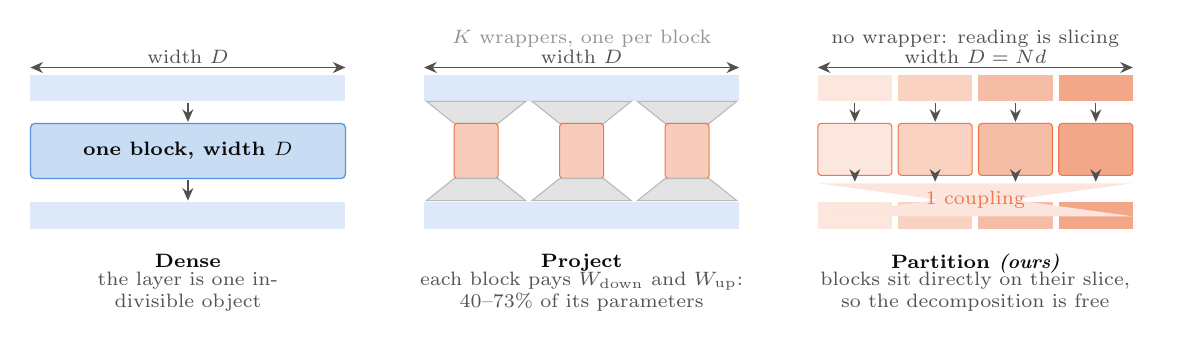
\begin{tikzpicture}[
  font=\footnotesize,
  >={Stealth[length=1.6mm,width=1.4mm]},
  stream/.style={draw=none, fill=denseblue!16},
  blkD/.style={draw=denseblue!80, line width=0.45pt, fill=denseblue!26,
               rounded corners=1.6pt},
  tile/.style={draw=mstorange!90, line width=0.4pt, rounded corners=1.2pt},
  tax/.style={draw=gray!55, line width=0.4pt, fill=gray!22},
  cplB/.style={draw=none, fill=mstorange!17},
  ar/.style={->, draw=ink2, line width=0.45pt},
  nm/.style={font=\scriptsize\bfseries, text=ink1},
  tag/.style={font=\scriptsize, text=ink2, inner sep=1pt},
  tagO/.style={font=\scriptsize, text=mstorange!90, inner sep=1pt},
  dimarr/.style={<->, draw=ink2, line width=0.35pt}
]
\def\W{4.0}
\def\barh{0.34}

% ===== (i) dense =====
\begin{scope}[shift={(0,0)}]
  \draw[dimarr] (0,2.62) -- (\W,2.62);
  \node[tag, anchor=south] at ({\W/2},2.63) {width $\dmodel$};
  \fill[stream] (0,2.19) rectangle (\W,{2.19+\barh});
  \draw[blkD] (0,1.21) rectangle (\W,1.91);
  \node[nm] at ({\W/2},1.56) {one block, width $\dmodel$};
  \fill[stream] (0,0.57) rectangle (\W,{0.57+\barh});
  \draw[ar] ({\W/2},2.17) -- ({\W/2},1.93);
  \draw[ar] ({\W/2},1.19) -- ({\W/2},0.93);
  \node[nm, anchor=north] at ({\W/2},0.37) {Dense};
  \node[tag, anchor=north, text width=40mm, align=center] at ({\W/2},0.07)
       {the layer is one indivisible object};
\end{scope}

% ===== (ii) project =====
\begin{scope}[shift={(5.0,0)}]
  \draw[dimarr] (0,2.62) -- (\W,2.62);
  \node[tag, anchor=south] at ({\W/2},2.63) {width $\dmodel$};
  \fill[stream] (0,2.19) rectangle (\W,{2.19+\barh});
  \foreach \k in {0,1,2} {
    \pgfmathsetmacro{\cx}{0.66+\k*1.34}
    \fill[tax] ({\cx-0.63},2.19) -- ({\cx+0.63},2.19) -- ({\cx+0.28},1.91)
               -- ({\cx-0.28},1.91) -- cycle;
    \draw[tile, fill=mstorange!34] ({\cx-0.28},1.21) rectangle ({\cx+0.28},1.91);
    \fill[tax] ({\cx-0.28},1.21) -- ({\cx+0.28},1.21) -- ({\cx+0.63},0.93)
               -- ({\cx-0.63},0.93) -- cycle;
  }
  \fill[stream] (0,0.57) rectangle (\W,{0.57+\barh});
  \node[tag, anchor=south, text=gray!85] at ({\W/2},2.83) {$K$ wrappers, one per block};
  \node[nm, anchor=north] at ({\W/2},0.37) {Project};
  \node[tag, anchor=north, text width=44mm, align=center] at ({\W/2},0.07)
       {each block pays $W_{\mathrm{down}}$ and $W_{\mathrm{up}}$:\\
        40--73\% of its parameters};
\end{scope}

% ===== (iii) partition =====
\begin{scope}[shift={(10.0,0)}]
  \draw[dimarr] (0,2.62) -- (\W,2.62);
  \node[tag, anchor=south] at ({\W/2},2.63) {width $\dmodel=\nsub\dsub$};
  \foreach \k in {0,1,2,3} {
    \pgfmathsetmacro{\lx}{\k*1.02}
    \pgfmathsetmacro{\sh}{int(16+\k*14)}
    \fill[mstorange!\sh] (\lx,2.19) rectangle ({\lx+0.94},{2.19+\barh});
    \draw[tile, fill=mstorange!\sh] (\lx,1.25) rectangle ({\lx+0.94},1.91);
    \draw[ar] ({\lx+0.47},2.17) -- ({\lx+0.47},1.93);
    \draw[ar] ({\lx+0.47},1.23) -- ({\lx+0.47},1.17);
    \draw[ar] ({\lx+0.47},0.71) -- ({\lx+0.47},0.67);
    \fill[mstorange!\sh] (\lx,0.57) rectangle ({\lx+0.94},{0.57+\barh});
  }
  \node[tag, anchor=south] at ({\W/2},2.83) {no wrapper: reading is slicing};
  \fill[cplB] (0,1.15) -- (\W,1.15) -- ({\W/2+0.47},0.94) -- ({\W/2-0.47},0.94) -- cycle;
  \fill[cplB] ({\W/2-0.47},0.94) -- ({\W/2+0.47},0.94) -- (\W,0.73) -- (0,0.73) -- cycle;
  \node[tagO] at ({\W/2},0.94) {1 coupling};
  \node[nm, anchor=north] at ({\W/2},0.37) {Partition~\itshape(ours)};
  \node[tag, anchor=north, text width=44mm, align=center] at ({\W/2},0.07)
       {blocks sit directly on their slice,\\ so the decomposition is free};
\end{scope}
\end{tikzpicture}
}
\end{center}
\caption{Three ways to make a transformer block narrow, all drawn at the same
total width $\dmodel$. Projecting into a narrow block costs a
$W_{\mathrm{down}}$/$W_{\mathrm{up}}$ wrapper on \emph{every} block. Partitioning
costs nothing, because each block sits directly on its own slice of the stream
and the $\nsub$ slices concatenated are the representation. The single coupling
that replaces the wrappers is detailed in Figure~\ref{fig:arch}.}
\label{fig:threeways}
\end{figure}

We ask whether the projection can be removed rather than amortized. Our answer is
a change of viewpoint: instead of projecting a full-width residual stream
\emph{into} narrow blocks, let the narrow blocks \emph{be} the residual stream.
If a layer holds $\nsub$ sub-transformers of width $\dsub = \dmodel/\nsub$, and
sub-transformer $i$ owns channels $[i\dsub, (i{+}1)\dsub)$ of the representation,
then reading and writing are free: they are slicing and concatenation. The
decomposition costs nothing, and what remains to be designed is only how the
sub-transformers communicate.

Our contributions:

\begin{enumerate}
\item \textbf{A projection-free layer decomposition.} MST partitions the residual
stream into $\nsub$ sub-streams processed by independent width-$\dsub$
transformers, coupled once per layer by a routed bottleneck
(Section~\ref{sec:method}). Per-layer matmul parameters fall from $12\dmodel^2$ to
$3.75\dmodel^2$ at $\nsub{=}4$, while attention FLOPs and KV cache are preserved
\emph{exactly by construction}, not approximately.

\item \textbf{Pareto dominance without sparsity.} On a compute-optimal ladder from
199M to 914M parameters, MST dominates a strong dense baseline on total
parameters, inference FLOPs per token, and total training compute simultaneously
(Section~\ref{sec:results}). Unlike MoE and MoL, MST is dense: all
sub-transformers are active for all tokens, so the parameter win is not traded
against active compute.

\item \textbf{The optimization of partitioned weights matters as much as the
architecture.} A naively-trained partition suffers a $7.2\times$ imbalance in
per-sub gradient norm and cross-sub contamination in the orthogonalizing
optimizer. Two fixes, per-sub gradient-norm equalization and block-diagonal
Newton--Schulz, together with a widened transition bottleneck, recover
\PH~\bpb\ at $\dmodel{=}512$ (Section~\ref{sec:ablations}).

\item \textbf{Coupling is necessary; its topology is not.} Removing the learned
transition costs 0.039~\bpb, yet eleven distinct attempts to enrich it
(nonlinear, gated, MLP, bilinear, per-slice routed, multi-layer lookback,
cross-sub gating, cross-sub KV injection, low-rank query modulation, feature
cycling, and a global residual stream) all fail to improve on it
(Section~\ref{sec:ablations}). This is an independent dense-architecture analogue
of the routing-equifinality result of \citet{ternovtsii2026equifinality}.
\end{enumerate}

% =========================================================================
\section{Related Work}
% =========================================================================

\paragraph{Narrow parallel blocks.} MoL \citep{ternovtsii2026mol} is the closest
work and the sharpest contrast. It replaces full-width blocks with $K$ thin
transformer blocks at reduced $d_{\text{thin}}$, selected per token by top-$k$
routing, and adds a shared full-attention block because sparse dispatch leaves
each routed block seeing only a fraction of the sequence. The design is motivated
by the same observation as ours, that the layer need not be monolithic, but it
answers differently on three counts. Its thin blocks read from and write to a
full-width residual stream, so each carries a $W_{\text{down}}$/$W_{\text{up}}$
wrapper costing 40--73\% of the block; it recovers that cost through sparsity,
activating $k$ of $K$ blocks; and it substitutes linear attention in the routed
blocks. The consequences are visible in its own results: at 1.3B, MoL leads an
iso-active dense baseline by 0.49 PPL but trails an iso-\emph{total} one by 3.01
PPL, and trains 1.9--2.3$\times$ slower. MST removes the wrapper instead of
amortizing it, stays dense, and keeps softmax attention throughout, which is why
it can be compared on total parameters at all. UoE \citep{yang2025uoe}
decomposes attention and MLP into expert groups with hierarchical routing, and
shares MoL's reliance on a full-width stream and on sparsity.

\paragraph{Residual-stream structure.} Hyper-Connections
\citep{hyperconnections2025, xie2026mhc} expand the residual into $n$
\emph{full-width} streams to improve optimization, at roughly $n\times$ residual
memory; AltUp \citep{baykal2023altup} widens the token representation and updates
one block per layer; Multi-Stream Transformers \citep{burtsev2021multistream}
split an encoder into parallel streams merged at the end. All of these
\emph{widen}. MST \emph{narrows} $\nsub$ streams to $\dmodel/\nsub$ and spends
the saving on depth. Concurrent work on FFN shape \citep{shape2026} and
channelized architectures \citep{dualstream2026} restructures within a layer but
leaves the residual width convention intact.

\paragraph{Partial partitions.} MH-MoE \citep{wu2024mhmoe} splits tokens into
sub-tokens routed to different experts and FlashMHF \citep{zhang2026flashmhf}
builds parallel narrow sub-networks inside the FFN; both are FFN-only and re-merge
within the layer. Layer-level modularity \citep{raposo2024mod, csordas2024moeut,
bae2025mor} changes which full-width blocks execute rather than their width. MST
partitions attention as well, and the partition persists across the full depth.

\paragraph{Structured matrices and attention spans.} An MST layer is by
construction a block-diagonal weight matrix with $\nsub$ blocks plus a low-rank
cross-block correction, placing it in the family of Monarch \citep{dao2022monarch}
and BLAST \citep{lee2024blast}, but applied to a whole layer rather than to
individual linear maps and with a learned, input-dependent correction. Assigning
different context windows to different heads or layers is likewise established
\citep{sukhbaatar2019adaptive, beltagy2020longformer, fu2024moa, zhang2025mswa};
MST lifts it from the head to the stream, so a window governs a block's attention,
its FFN and its slice of the residual jointly.

% =========================================================================
\section{Method}
\label{sec:method}
% =========================================================================

\begin{figure}[t]
\begin{center}
\resizebox{\textwidth}{!}{% MST architecture figure. \input inside a figure environment.
% Requires tikz + libraries positioning, arrows.meta, calc, decorations.pathreplacing.
% Requires colors mstorange, denseblue, ink1, ink2 from the preamble.
%
% Read bottom to top, like a standard transformer block diagram. Every box is
% named. Colour encodes width and nothing else: BLUE operates at D, ORANGE at d.
% Repetition is the "x L" bracket rather than something drawn out.
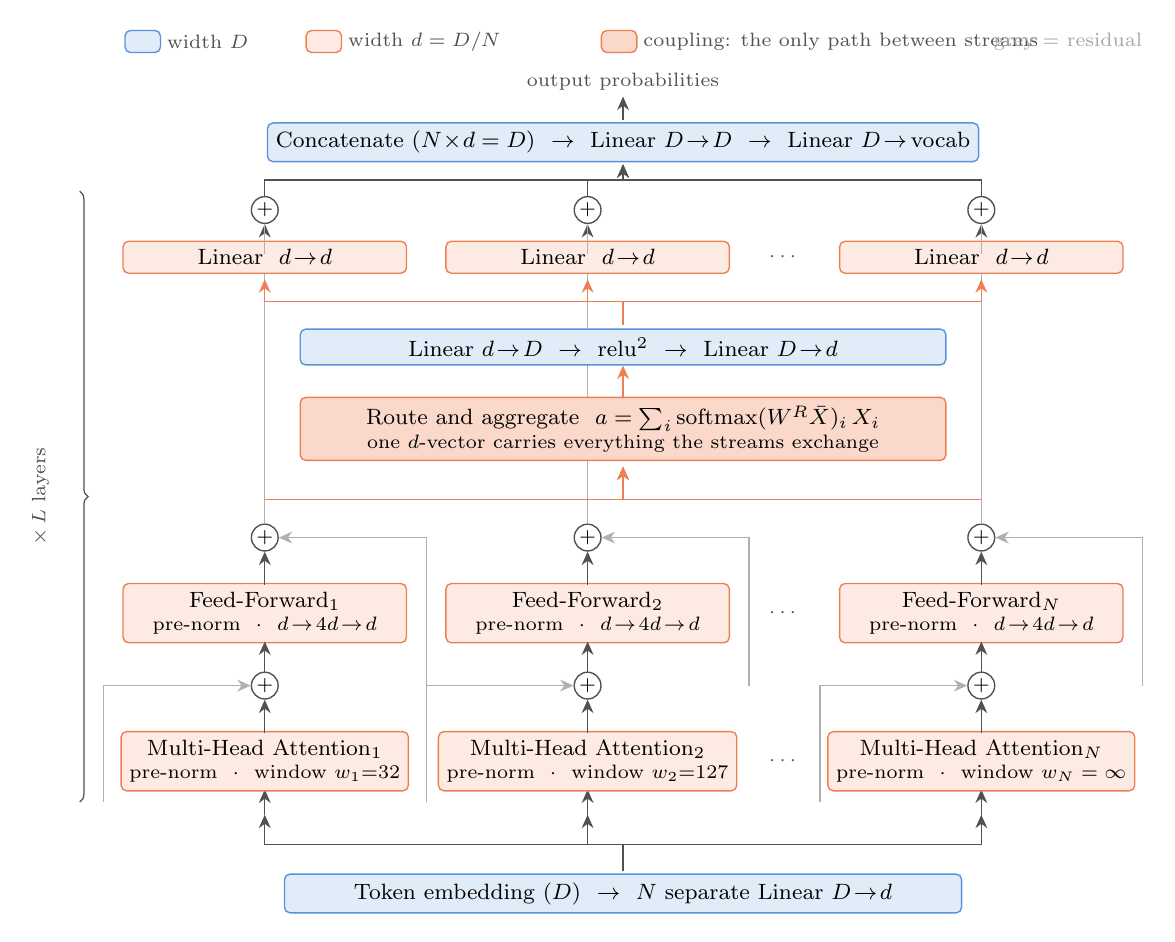
\begin{tikzpicture}[
  font=\footnotesize,
  >={Stealth[length=1.7mm,width=1.5mm]},
  boxD/.style={draw=denseblue!80, line width=0.5pt, fill=denseblue!14,
               rounded corners=2pt, align=center, inner sep=3pt},
  boxd/.style={draw=mstorange!85, line width=0.5pt, fill=mstorange!14,
               rounded corners=2pt, align=center, inner sep=3pt},
  boxc/.style={draw=mstorange!85, line width=0.5pt, fill=mstorange!26,
               rounded corners=2pt, align=center, inner sep=3pt},
  ar/.style={->, draw=ink2, line width=0.5pt},
  arS/.style={->, draw=gray!62, line width=0.45pt},
  arO/.style={->, draw=mstorange!85, line width=0.5pt},
  plus/.style={draw=ink2, line width=0.5pt, circle, fill=white, inner sep=0pt,
               minimum size=3.4mm, font=\scriptsize},
  tag/.style={font=\scriptsize, text=ink2, inner sep=1.5pt},
  tagO/.style={font=\scriptsize, text=mstorange!95, inner sep=1.5pt},
  brc/.style={decorate, decoration={brace, amplitude=3pt}, draw=ink2,
              line width=0.45pt}
]

% ==== column geometry
\def\ca{2.20}   \def\cb{6.30}   \def\cc{11.30}   % stream 1, stream 2, stream N
\def\bw{36mm}
\def\xl{0.40}   \def\xr{13.10}
\pgfmathsetmacro{\cmid}{(\xl+\xr)/2}
\def\xel{8.80}                                    % x of the elision
\def\sk{2.05}                                     % residual offset from column centre

% ==== bottom: embedding and the split
\node[boxD, minimum width=86mm] (emb) at (\cmid,0.30)
     {Token embedding ($\dmodel$)\ \ $\to$\ \ $\nsub$ separate Linear $\dmodel\!\to\!\dsub$};
\foreach \c/\i in {\ca/1, \cb/2, \cc/N} {
  \draw[ar] (\cmid,0.58) -- (\cmid,0.92) -- (\c,0.92) -- (\c,1.30);
}

% ==== per-stream sublayers
\foreach \c/\i/\w in {\ca/1/{$w_1{=}32$}, \cb/2/{$w_2{=}127$}, \cc/N/{$w_{\nsub}=\infty$}} {
  \draw[ar] (\c,1.30) -- (\c,1.62);
  \node[boxd, minimum width=\bw] (at\i) at (\c,1.98)
       {Multi-Head Attention$_{\i}$\\[-1pt]\scriptsize pre-norm\ \ $\cdot$\ \ window \w};
  \node[plus] (p\i) at (\c,2.94) {$+$};
  \draw[ar] (\c,2.34) -- (p\i);
  \draw[arS] ({\c-\sk},1.46) -- ({\c-\sk},2.94) -- (p\i);

  \node[boxd, minimum width=\bw] (ff\i) at (\c,3.86)
       {Feed-Forward$_{\i}$\\[-1pt]\scriptsize pre-norm\ \ $\cdot$\ \ $\dsub\!\to\!4\dsub\!\to\!\dsub$};
  \draw[ar] (p\i) -- (\c,3.50);
  \node[plus] (q\i) at (\c,4.82) {$+$};
  \draw[ar] (\c,4.22) -- (q\i);
  \draw[arS] ({\c+\sk},2.94) -- ({\c+\sk},4.82) -- (q\i);
}

% ==== the stream continues straight through the coupling
% drawn FIRST so the coupling boxes sit on top of it: the line visibly passes
% behind the shared module and re-emerges, which is what a residual does.
\foreach \c/\i in {\ca/1, \cb/2, \cc/N} {
  \draw[draw=gray!62, line width=0.45pt] (\c,5.00) -- (\c,8.42);
}

% ==== coupling: gather, bottleneck, scatter
\foreach \c/\i in {\ca/1, \cb/2, \cc/N} {
  \draw[arO] (\c,5.30) -- (\cmid,5.30) -- (\cmid,5.72);
}
\node[boxc, minimum width=82mm] (rt) at (\cmid,6.20)
     {Route and aggregate\ \ $a=\sum_i \mathrm{softmax}(W^{R}\bar{X})_i\,X_i$\\[-1pt]
      \scriptsize one $\dsub$-vector carries everything the streams exchange};
\node[boxD, minimum width=82mm] (bn) at (\cmid,7.24)
     {Linear $\dsub\!\to\!\dmodel$\ \ $\to$\ \ $\mathrm{relu}^2$\ \ $\to$\ \ Linear $\dmodel\!\to\!\dsub$};
\draw[arO] (rt) -- (bn);

\foreach \c/\i in {\ca/1, \cb/2, \cc/N} {
  \draw[arO] (\cmid,7.52) -- (\cmid,7.82) -- (\c,7.82) -- (\c,8.10);
  \node[boxd, minimum width=\bw] (rd\i) at (\c,8.38) {Linear\ \ $\dsub\!\to\!\dsub$};
  \node[plus] (r\i) at (\c,8.98) {$+$};
  \draw[ar] (\c,8.64) -- (r\i);
  \draw[draw=gray!62, line width=0.45pt] (\c,8.42) -- (r\i);
}

% ==== repetition bracket
\draw[brc] ({\xl-0.55},9.22) -- ({\xl-0.55},1.46);
\node[tag, rotate=90, anchor=south] at ({\xl-0.88},5.34) {$\times\,L$ layers};

% ==== top: recombine and predict
\foreach \c/\i in {\ca/1, \cb/2, \cc/N} {
  \draw[ar] (\c,9.16) -- (\c,9.36) -- (\cmid,9.36) -- (\cmid,9.56);
}
\node[boxD, minimum width=86mm] (cat) at (\cmid,9.84)
     {Concatenate ($\nsub\!\times\!\dsub=\dmodel$)\ \ $\to$\ \ Linear $\dmodel\!\to\!\dmodel$\ \ $\to$\ \ Linear $\dmodel\!\to\!$ vocab};
\draw[ar] (\cmid,10.12) -- (\cmid,10.42);
\node[tag, anchor=south] at (\cmid,10.44) {output probabilities};

% ==== stream captions and elision
\foreach \y in {1.98, 3.86, 8.38} { \node[tag] at (\xel,\y) {$\cdots$}; }

% ==== legend
\node[boxD, minimum width=4.5mm, minimum height=2.8mm, inner sep=1pt]
     at ({\xl+0.25},11.12) {};
\node[tag, anchor=west] at ({\xl+0.50},11.12) {width $\dmodel$};
\node[boxd, minimum width=4.5mm, minimum height=2.8mm, inner sep=1pt]
     at ({\xl+2.55},11.12) {};
\node[tag, anchor=west] at ({\xl+2.80},11.12) {width $\dsub=\dmodel/\nsub$};
\node[boxc, minimum width=4.5mm, minimum height=2.8mm, inner sep=1pt]
     at ({\xl+6.30},11.12) {};
\node[tag, anchor=west] at ({\xl+6.55},11.12)
     {coupling: the only path between streams};
\node[tag, anchor=west, text=gray!70] at ({\xl+11.00},11.12) {grey = residual};

\end{tikzpicture}
}
\end{center}
\caption{One MST layer, read bottom to top. Colour encodes width and nothing
else: blue operates at $\dmodel$, orange at $\dsub=\dmodel/\nsub$. The $\nsub$
streams run ordinary transformer sublayers in parallel and never read each
other's channels; the coupling is the only path between them, and everything
they exchange passes through the single $\dsub$-vector $a$. Grey lines are
residual connections, which carry each stream past the coupling unchanged.}
\label{fig:arch}
\end{figure}

\paragraph{Notation.} $\dmodel$ is the model width, $\nsub$ the number of
sub-transformers, $\dsub=\dmodel/\nsub$ the sub width, and $L$ the depth. The
state at layer $\ell$ is $H^{(\ell)}\in\mathbb{R}^{B\times T\times \nsub\times \dsub}$;
its flattening over the last two axes is the ordinary $\dmodel$-dimensional
residual stream. We write $X_i \in \mathbb{R}^{\dsub}$ for the $i$-th sub-state at
a given token and suppress the batch and time axes throughout. Each
sub-transformer uses $n_h$ heads of dimension $d_h$ with $n_h d_h = \dsub$.

\subsection{The layer}

\paragraph{Per stream: nothing new.} Sub-transformer $i$ owns $X_i$ and no other
channel. It runs an ordinary pre-norm transformer block at width $\dsub$, with its
own attention window $w_i$, RoPE \citep{su2021roformer} and QK-norm:
%
\begin{equation}
X_i \;\leftarrow\; X_i + W^{O}_i\,\mathrm{Attn}_{w_i}\!\big(W^{Q}_i\tilde{X}_i,\ W^{K}_i\tilde{X}_i,\ W^{V}_i\tilde{X}_i\big),
\qquad
X_i \;\leftarrow\; X_i + W^{F2}_i\,\mathrm{relu}^2\!\big(W^{F1}_i\tilde{X}_i\big),
\end{equation}
%
where $\tilde{X}_i = \mathrm{RMSNorm}(X_i)$ is recomputed before each sublayer.
This is deliberately unremarkable: it is the dense baseline's block with $\dmodel$
replaced by $\dsub$ everywhere. Because no term reads a channel that sub $i$ does
not own, the $\nsub$ blocks together form a block-diagonal factorization of one
$\dmodel$-width layer rather than $\nsub$ copies of a smaller model.

\paragraph{Coupling: the whole mechanism, in one line.} The streams exchange
information exactly once per layer. Everything they say to each other passes
through a single $\dsub$-dimensional vector:
%
\begin{equation}
\label{eq:coupling}
X_i \;\leftarrow\; X_i \;+\;
\overbrace{W^{D}_i}^{\substack{\text{scatter}\\ 1\,\to\,\nsub}}
\underbrace{W^{\downarrow}\,\mathrm{relu}^2\Big(W^{\uparrow}}_{\substack{\text{bottleneck}\\ \dsub\,\to\,\dmodel\,\to\,\dsub}}
\overbrace{\textstyle\sum_{j} p_j\,\tilde{X}_j}^{\substack{\text{aggregate}\\ \nsub\,\to\,1}}\Big),
\qquad
p \;=\; \mathrm{softmax}\Big(W^{R}\,\tfrac{1}{\nsub}\textstyle\sum_{j}\tilde{X}_j\Big).
\end{equation}
%
Read right to left, Eq.~\ref{eq:coupling} is the hourglass of
Figure~\ref{fig:arch}: $\nsub$ streams collapse to one $\dsub$-vector, that vector
is widened to $\dmodel$ for a single nonlinearity and squeezed back to $\dsub$, and
$\nsub$ distinct read-out matrices deliver it. Parameter shapes and counts are in
Appendix~\ref{app:budget}.

Three consequences follow directly from the form of Eq.~\ref{eq:coupling}.

\emph{(i) The router selects nothing.} $p$ lies in the simplex over
\emph{sub-transformers}, not over tokens-to-experts. Every stream runs for every
token, so MST has no sparse dispatch, no capacity factor, and no dropped tokens. A
light load-balancing term $\alpha\nsub\sum_i \bar{p}_i^2$ with $\alpha{=}0.01$
\citep{fedus2022switch} is minimized at uniform $p$.

\emph{(ii) The $\nsub$ read-outs are what break the symmetry.} Every stream
receives the same vector. Through a shared $W^{D}$ they would receive identical
messages and could diverge only through initialization noise. The distinct
$W^{D}_i$ make the message stream-specific, and they are the cheapest term in the
layer (Appendix~\ref{app:budget}).

\emph{(iii) The layer is exactly the identity at step 0.} $W^{O}_i$, $W^{F2}_i$
and $W^{\downarrow}$ are zero-initialized and $W^{R}$ starts at zero, so every
residual branch contributes nothing and $p$ is exactly uniform. Training begins
from a well-conditioned deep identity, not from a random partitioned map.

\paragraph{The head budget is conserved.} Each sub spends $n_h d_h = \dsub$ on
attention, so the layer spends $\nsub\dsub = \dmodel$, exactly as a dense layer
does. This one identity is why attention FLOPs and KV cache are preserved while
only the matmul parameters shrink (Section~\ref{sec:cost}). Our dense baseline
uses $d_h{=}128$; MST uses $d_h{=}128/\nsub{=}32$ with $\nsub$ times as many heads.

\subsection{Multi-scale sub-windows}
\label{sec:windows}

Sub-transformer $i$ attends with a causal sliding window $w_i$ spaced
geometrically from $w_{\min}{=}32$ to full context, the last sub always
unrestricted. For $\nsub{=}4$ at $T{=}2048$ this gives
$w=(32,\,127,\,511,\,\infty)$. This is the only component of MST that supplies an
\emph{a priori} reason for sub-transformers to differ; every other source of
differentiation is symmetry breaking through $W^{D}_i$ and initialization.

The assignment is close to FLOP-neutral, so it is a prior rather than a shortcut.
Summed effective context is $32+127+511+2048=2718$ per layer against
$4\times704=2816$ for the dense baseline's \texttt{SSSL} layer-alternating
pattern, a 3.5\% reduction.

\subsection{Optimizing partitioned weights}
\label{sec:optim}

The $\nsub$ matrices of each type are stored fused as one
$(\nsub\!\cdot\!\text{out})\times\text{in}$ tensor and applied with a batched
matrix multiply. That is an implementation detail for throughput, but it exposes
two training problems that a dense model does not have.

\textbf{Gradient imbalance.} Measured on the $\nsub{=}4$ model, per-sub gradient
norms differ by $7.2\times$: sub 0 receives 55\% of the total and sub 3 receives
7.6\%. The mechanism is a feedback loop through the concatenating output head,
which weights one sub more, which trains it faster, which weights it more still.
We equalize with a backward hook that views the fused gradient as
$(\nsub,\text{out},\text{in})$ and rescales each sub to the mean norm. Only
magnitudes are touched; directions are left alone.

\textbf{Cross-sub contamination in Muon.} Muon orthogonalizes the update via a
Newton--Schulz / Polar-Express iteration \citep{jordan2024muon, amsel2025polar}.
Applied to the fused tensor it mixes gradient directions belonging to different
sub-transformers, which is exactly what the partition is designed to keep apart.
We run the iteration independently on each of the $\nsub$ blocks. Because Muon
scales its step by $\max(1,\text{rows}/\text{cols})^{1/2}$, blocking also divides
the effective learning rate on the fused attention tensors by $\sqrt{\nsub}$; we
restore it with a per-sub multiplier of $\sqrt{\nsub}$, which simultaneously
corrects the $\mu$P \citep{yang2021mup} mismatch between a $\dmodel$-tuned rate
and $\dsub$-wide matrices. The two interventions are therefore coupled and we
ablate them jointly (Section~\ref{sec:ablations}).

\subsection{Cost accounting}
\label{sec:cost}



\textbf{Parameters.} Summing the components of Eq.~\ref{eq:coupling} and the
per-stream sublayers (Appendix~\ref{app:budget} gives the term-by-term budget),
%
\begin{equation}
\label{eq:budget}
\underbrace{\tfrac{12\dmodel^2}{\nsub}}_{\text{$\nsub$ sub-transformers}}
\;+\;
\underbrace{\tfrac{3\dmodel^2}{\nsub}}_{\text{coupling}}
\;=\;
\frac{15\dmodel^2}{\nsub}
\quad\text{per layer, against}\quad
12\dmodel^2\ \text{dense,}
\end{equation}
%
a reduction of $0.8\nsub$ rather than $\nsub$: the coupling consumes a quarter of
what the partition saves. It is nonetheless far cheaper than a projection
wrapper, which costs $2\dmodel\dsub$ \emph{per block} rather than once per layer.

\textbf{Attention FLOPs and KV cache.} A sub contributes
$12\,n_h d_h\,T_{\mathrm{eff}} = 12\,\dsub\,T_{\mathrm{eff}}$ per token per layer;
summed over $\nsub$ subs this is $12\,\dmodel\,T_{\mathrm{eff}}$, the dense value
exactly. The KV cache is $\nsub\dsub = \dmodel$ per layer, again exactly dense.
MST therefore takes its saving entirely from matmul parameters and inherits
neither an attention advantage nor an attention penalty, which is what makes the
FLOPs-per-token axis of Section~\ref{sec:results} a clean comparison.

\textbf{Value embeddings.} Per-layer value embeddings \citep{zhou2024resformer} in
MST live at width $\dsub$ and are shared across subs with per-sub gates, so they
are $\nsub\times$ smaller than the dense baseline's. Since the dense baseline
spends 44\% of its total parameters on value embeddings at $L{=}24$, we report
transformer-matrix parameters alongside total parameters throughout
(Table~\ref{tab:cost}) so that this effect can be separated from the layer
decomposition itself.

% =========================================================================
\section{Experimental setup}
\label{sec:experiments}
% =========================================================================

\textbf{Baseline.} Our dense baseline is not a vanilla transformer. It is a
speedrun-tuned decoder \citep{karpathy2025nanochat} with RMSNorm pre-norm, RoPE,
QK-norm, $\mathrm{relu}^2$ FFN, per-layer value embeddings, layer-alternating
sliding-window attention, logit soft-capping, learned per-layer residual scalars,
Muon for matrices with AdamW for embeddings and scalars, $\mu$P learning-rate
transfer, and a batch-size schedule following \citet{bergsma2025powerlines}. MST
changes only the layer structure; every other component, hyper-parameter and
schedule is shared.

\textbf{Ladder.} $\dmodel = 64L$ rounded up to a multiple of 128; $\nsub{=}4$;
$T{=}2048$; vocabulary 32{,}768. Both arms are trained at 10.5 tokens per scaling
parameter (transformer matrices plus output head), so each model receives its own
compute-optimal budget \citep{hoffmann2022chinchilla}; MST consequently trains on
fewer tokens than dense at equal depth. Data is a filtered web corpus
\citep{penedo2024fineweb}, single epoch.

\textbf{Metric.} Bits per byte on held-out data, which is invariant to tokenizer
vocabulary.

% =========================================================================
\section{Results}
\label{sec:results}
% =========================================================================

\begin{table}[t]
\caption{Cost and quality. MST is $\nsub{=}4$ with all components of
Section~\ref{sec:method}. Dense is the matched baseline at the same $\dmodel = 64L$
ladder. ``Matrices'' excludes embeddings and value embeddings.}
\label{tab:cost}
\begin{center}
\begin{small}
\begin{tabular}{llrrrrr}
\toprule
Model & $L$ & Total params & Matrices & FLOPs/token & Train FLOPs & \bpb $\downarrow$ \\
\midrule
\multirow{9}{*}{MST}
 & 8  & 58{,}726{,}416   & 8.4M    & 1.844e8 & 4.875e16 & 1.0510$^\ddagger$ \\
 & 9  & 82{,}809{,}618   & 14.7M   & 2.607e8 & 9.752e16 & 1.0000$^\ddagger$ \\
 & 16 & 199{,}254{,}048  & 65.0M   & 7.251e8 & 7.507e17 & 0.8810 \\
 & 18 & 252{,}696{,}996  & 92.3M   & 9.492e8 & 1.296e18 & 0.8544 \\
 & 20 & 314{,}938{,}920  & 126.2M  & 1.218e9 & 2.150e18 & 0.8349 \\
 & 22 & 386{,}717{,}100  & 167.6M  & 1.535e9 & 3.444e18 & 0.8104 \\
 & 24 & 468{,}768{,}816  & 217.1M  & 1.905e9 & 5.350e18 & 0.7946 \\
 & 26 & 561{,}831{,}348  & 275.6M  & 2.333e9 & 8.087e18 & 0.7804 \\
 & 32 & 914{,}456{,}640  & 511.8M  & 4.008e9 & 2.436e19 & 0.7434 \\
\midrule
\multirow{11}{*}{Dense}
 & 8  & 125{,}829{,}648    & 25.2M   & 2.863e8 & 1.261e17 & 0.9691 \\
 & 12 & 286{,}262{,}424    & 84.9M   & 7.385e8 & 8.537e17 & 0.9030 \\
 & 14 & 399{,}115{,}836    & 134.9M  & 1.101e9 & 1.899e18 & 0.8688 \\
 & 16 & 536{,}872{,}992    & 201.3M  & 1.548e9 & 3.817e18 & 0.8364 \\
 & 18 & 701{,}893{,}188    & 286.7M  & 2.134e9 & 7.269e18 & 0.8131 \\
 & 20 & 896{,}535{,}720    & 393.2M  & 2.827e9 & 1.292e19 & 0.7906 \\
 & 22 & 1{,}123{,}159{,}884 & 523.4M & 3.694e9 & 2.209e19 & 0.7714 \\
 & 24 & 1{,}384{,}124{,}976 & 679.5M & 4.690e9 & 3.594e19 & 0.7545 \\
 & 26 & 1{,}681{,}790{,}292 & 863.9M & 5.894e9 & 5.684e19 & 0.7382 \\
 & 28 & 2{,}018{,}515{,}128 & 1079.0M & 7.250e9 & 8.661e19 & 0.7246 \\
 & 30 & 2{,}396{,}658{,}780 & 1327.1M & 8.847e9 & 1.291e20 & 0.7120 \\
\bottomrule
\end{tabular}
\end{small}
\end{center}
$^\ddagger$\,below the amortization threshold; excluded from the fits of
Table~\ref{tab:fits} and reported as a sensitivity in Section~\ref{sec:limitations}.
All cost columns are recomputed from a single implementation at one commit, so the
two arms are directly comparable; the token budget is $10.5$ tokens per scaling
parameter and Train FLOPs is FLOPs/token $\times$ tokens.
\end{table}

\subsection{Pareto dominance}

\begin{figure}[t]
\begin{center}
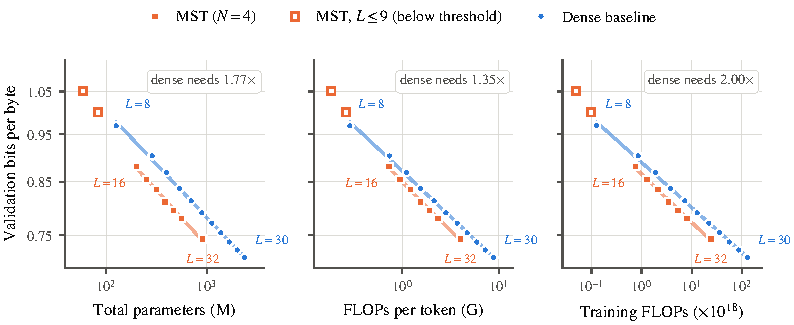
\includegraphics[width=\textwidth]{fig_scaling.pdf}
\end{center}
\caption{MST lies below the dense scaling curve on all three cost axes. Points are
measured runs; lines are power-law fits (Table~\ref{tab:fits}). Hollow markers are
MST models below the amortization threshold, which are excluded from the MST fit.
Each panel states the multiplier a dense model needs to reach the same
bits-per-byte, averaged over $L\!\in\![16,32]$.}
\label{fig:pareto}
\end{figure}

Figure~\ref{fig:pareto} shows MST below the
dense curve on all three axes over the entire measured range. Table~\ref{tab:ratio}
quantifies the gap by inverting the dense fit: for each MST model we report the
resource a dense model would require to reach the same \bpb.

\begin{table}[t]
\caption{Resource multiplier a dense model needs to match each MST model, obtained
by inverting the dense power-law fit. The multiplier is stable across the range.}
\label{tab:ratio}
\begin{center}
\begin{small}
\begin{tabular}{lrrrrrrrr}
\toprule
MST $L$ & 16 & 18 & 20 & 22 & 24 & 26 & 32 & \textbf{mean} \\
\midrule
Total parameters & 1.66 & 1.74 & 1.73 & 1.86 & 1.84 & 1.82 & 1.75 & \textbf{1.77}$\times$ \\
FLOPs / token    & 1.22 & 1.30 & 1.30 & 1.42 & 1.42 & 1.41 & 1.39 & \textbf{1.35}$\times$ \\
Training FLOPs   & 1.64 & 1.86 & 1.85 & 2.22 & 2.20 & 2.16 & 2.08 & \textbf{2.00}$\times$ \\
\bottomrule
\end{tabular}
\end{small}
\end{center}
\end{table}

\subsection{Scaling exponents}

Fitting $\bpb = a x^{b}$ (Table~\ref{tab:fits}), MST's exponents are marginally
steeper on all three axes, but the difference is within fit uncertainty for seven
points and we do \emph{not} claim a scaling-exponent advantage. The defensible
statement is that the multiplier of Table~\ref{tab:ratio} is approximately
constant over a $4.6\times$ span of parameters and a $32\times$ span of training
compute. Including models below 100M ($L\le9$) would widen the exponent gap
substantially, but those points lie \emph{above} the dense curve on the compute
axes and steepen the fit artificially; we report that crossover in
Section~\ref{sec:limitations} rather than fitting through it.

\begin{table}[t]
\caption{Power-law fits $\bpb = a x^{b}$, MST $L\!\in\![16,32]$ and dense $L\!\in\![12,30]$.}
\label{tab:fits}
\begin{center}
\begin{small}
\begin{tabular}{lcccc}
\toprule
Axis $x$ & Dense $a$, $b$ & $R^2$ & MST $a$, $b$ & $R^2$ \\
\midrule
Total parameters & $7.291\,x^{-0.1077}$ & 0.998 & $7.446\,x^{-0.1119}$ & 0.996 \\
FLOPs / token    & $5.904\,x^{-0.0923}$ & 0.998 & $6.713\,x^{-0.0997}$ & 0.996 \\
Training FLOPs   & $5.905\,x^{-0.0457}$ & 0.998 & $6.590\,x^{-0.0490}$ & 0.996 \\
\bottomrule
\end{tabular}
\end{small}
\end{center}
\end{table}

\subsection{Downstream transfer}

Perplexity gaps of this size need not translate into downstream ability, so we
evaluate zero-shot transfer against two dense reference points that bracket MST:
one matched on total parameters and one matched on FLOPs per token
(Table~\ref{tab:downstream}). \PH

\begin{table}[t]
\caption{Zero-shot accuracy (\%). MST is compared against a dense model matched on
total parameters and a dense model matched on FLOPs per token.}
\label{tab:downstream}
\begin{center}
\begin{small}
\begin{tabular}{lccc}
\toprule
Task & MST $L{=}32$ & Dense $L{=}20$ & Dense $L{=}22$ \\
     & (914M) & (iso-param) & (iso-FLOP) \\
\midrule
ARC-Easy (10-shot)      & 66.8 & \PH & \PH \\
PIQA (10-shot)          & 73.3 & \PH & \PH \\
HellaSwag (10-shot)     & 51.6 & \PH & \PH \\
Winograd (0-shot)       & 63.4 & \PH & \PH \\
LAMBADA (0-shot)        & 40.0 & \PH & \PH \\
OpenBook QA (0-shot)    & 40.0 & \PH & \PH \\
ARC-Challenge (10-shot) & 37.5 & \PH & \PH \\
\midrule
\textbf{CORE metric}    & \textbf{0.231} & \PH & \PH \\
\bottomrule
\end{tabular}
\end{small}
\end{center}
Seven of the 22 CORE tasks, chosen as those with meaningful headroom at this
scale; the CORE metric aggregates all 22. Tasks on which a model of this size
sits at chance (CommonsenseQA, WinoGrande, Jeopardy, BigBench repeat-copy) carry
no signal here and are deferred to Appendix~\ref{app:details}.
\TODO{dense columns pending: $L{=}20$ is $0.98\times$ MST total params, $L{=}22$
is $0.92\times$ MST FLOPs/token}
\end{table}

\subsection{Throughput, memory and hardware utilization}

FLOP counts are not wall-clock. MST trains $1.20\times$ faster than dense while
reaching less than half its utilization (Table~\ref{tab:speed}): it wins on
throughput by issuing $2.46\times$ fewer FLOPs, not by using the machine well.

\paragraph{The utilization gap has two distinct causes.} Measuring fused
attention in isolation, with the total attention width held constant and no MST
code in the loop, gives 171.9, 283.9 and 365.7 TFLOP/s at $d_h = 32$, $64$ and
$128$ (Figure~\ref{fig:kernels}). A partition into $\nsub$ streams forces
$d_h = 128/\nsub$, so at $\nsub{=}4$ a $2.13\times$ penalty on the attention
portion is intrinsic to the architecture given current kernels. The remainder is
ours: the layer issues $\nsub$ separate attention calls, one per stream, where a
single call over $\nsub n_h$ heads would compute the same thing whenever the
streams share a window, since attention is independent across heads. At $L{=}24$
that is 96 launches per forward pass where 24 would do. We report the measured
kernel penalty and do not claim to have eliminated the implementation cost.

\paragraph{Memory.} MST's peak memory is $8\%$ \emph{higher} than dense despite
$3.2\times$ fewer per-layer parameters. The cause is the batched formulation
rather than the partition: applying $\nsub$ stacked weight matrices requires a
permutation before the batched matrix multiply, which forces a contiguous copy of
a full activation tensor, and this happens for each of the six batched
projections per layer. Parameter count shrinks with $\nsub$; activation traffic
does not. The same extra data movement lowers arithmetic intensity, so the memory
overhead and the utilization gap share a cause rather than one explaining the
other.

\begin{table}[t]
\caption{Measured throughput and memory. Weights are randomly initialized;
these are architecture-level measurements and do not depend on training.}
\label{tab:speed}
\begin{center}
\begin{small}
\begin{tabular}{lccc}
\toprule
Measurement ($L{=}24$, H200) & MST & Dense & \\
\midrule
Training step, fwd+bwd (ms)     & \textbf{420.4} & 504.4 & MST $1.20\times$ faster \\
Achieved throughput (TFLOP/s)   & 297 & 609 & \\
Model FLOPs utilization (\%)    & 30.0 & 61.6 & dense $2.05\times$ higher \\
Peak memory (GB)                & 115.3 & 106.7 & MST $8\%$ higher \\
KV cache per layer              & $\dmodel$ & $\dmodel$ & identical by construction \\
\midrule
Decode latency (ms/token)       & \PH & \PH & \TODO{pending} \\
\bottomrule
\end{tabular}
\end{small}
\end{center}
Batch 32, $T{=}2048$, \texttt{torch.compile} enabled for both arms as in
training, minimum over 20 iterations. Weights are randomly initialised: these are
architecture-level measurements independent of the trained values.
\end{table}

\begin{figure}[t]
\begin{center}
\fbox{\parbox[c][2.4cm][c]{0.95\textwidth}{\centering \TODO{Fig.~3: (a) fused
attention throughput vs $d_h$ at constant total width: 171.9 / 283.9 / 365.7
TFLOP/s for $d_h=32/64/128$; (b) MST kernel-time breakdown.}}}
\end{center}
\caption{The utilization gap decomposes into a kernel effect and an
implementation cost. Fused attention at $d_h{=}32$, which $\nsub{=}4$ forces,
reaches only $2.13\times$ less throughput than at $d_h{=}128$ with the total
attention width held fixed and no MST code involved.}
\label{fig:kernels}
\end{figure}

Figure~\ref{fig:kernels}
attributes the utilization gap to the head-dimension
regime rather than to the architecture, and therefore identifies it as
implementation headroom.

% =========================================================================
\section{Ablations}
\label{sec:ablations}
% =========================================================================

Ablations are run at $L{=}8$ ($\dmodel{=}512$), where a full grid is affordable,
with three seeds per condition. A $L{=}16$ grid would cost roughly $40\times$ as
much and we did not run one.

\paragraph{Ablation transfer.} Small-scale ablations are only useful if their
conclusions survive at the scales the paper actually claims. We can test this
directly for the one intervention we measured at two depths: the full training
recipe of Section~\ref{sec:optim} applied to the plain partition. It preserves its
sign and, to within 15\%, its magnitude (Table~\ref{tab:transfer}). We take this as
evidence that the $L{=}8$ ordering is informative about $L{=}16$, while noting that
one intervention at two depths is a weak test and that we cannot rule out an
ablation whose sign flips with scale.

\begin{table}[t]
\caption{Ablation transfer. The one intervention measured at two depths keeps its
sign and approximate magnitude, which is the basis on which we run the remaining
ablations at $L{=}8$ only.}
\label{tab:transfer}
\begin{center}
\begin{small}
\begin{tabular}{lccc}
\toprule
Condition & $L{=}8$ (\bpb) & $L{=}16$ (\bpb) & \\
\midrule
Plain partition (no recipe)          & 1.0798 & 0.9057 & \\
\; + full recipe (Section~\ref{sec:optim}) & 1.0510 & 0.8810 & \\
\midrule
$\Delta$                              & $-0.0288$ & $-0.0247$ & \textbf{same sign, $0.86\times$ magnitude} \\
\bottomrule
\end{tabular}
\end{small}
\end{center}
\end{table}

\begin{table}[t]
\caption{Ablations at $L{=}8$, $\dmodel{=}512$, $\nsub{=}4$, mean $\pm$ s.d. over
3 seeds. Negative $\Delta$ is better.}
\label{tab:ablation}
\begin{center}
\begin{small}
\begin{tabular}{llcc}
\toprule
& Condition & \bpb & $\Delta$ \\
\midrule
\multirow{2}{*}{Controls}
 & Dense baseline ($d_h{=}128$)                & $0.9592\pm0.0002$ & n/a \\
 & Dense baseline, $d_h{=}32$ \emph{(head-dim control)} & $0.9760\pm0.0003$ & $+0.0168$ \\
\midrule
\multirow{3}{*}{Coupling}
 & No coupling (independent columns)           & \PH & \PH \\
 & Parameter-free mean coupling                & \PH & \PH \\
 & Routed bottleneck (ours)                    & \PH & n/a \\
\midrule
\multirow{4}{*}{Recipe}
 & Plain partition (no recipe)                 & \PH & \PH \\
 & \; + gradient equalization                  & \PH & \PH \\
 & \; + block-diagonal Muon \& per-sub LR      & \PH & \PH \\
 & \; + wide transition                        & \PH & \PH \\
\midrule
\multirow{2}{*}{Full}
 & All of the above                            & \PH & \PH \\
 & \; + multi-scale sub-windows (\textbf{MST}) & \PH & \PH \\
\midrule
\multirow{3}{*}{Granularity}
 & $\nsub{=}2$ & \PH & \PH \\
 & $\nsub{=}4$ & \PH & n/a \\
 & $\nsub{=}8$ & \PH & \PH \\
\bottomrule
\end{tabular}
\end{small}
\end{center}
\TODO{Tier-3 grid; the head-dim control is the load-bearing row}
Block-diagonal Muon and the per-sub learning rate are ablated as a unit because
blocking divides the effective rate by $\sqrt{\nsub}$ and the multiplier restores
it; the two separately, and the bottleneck-width sweep, are in
Appendix~\ref{app:extra}.
\end{table}

\paragraph{Granularity.} $\nsub{=}4$ substantially outperforms $\nsub{=}8$ at
equal $\dmodel$ (\PH\ versus \PH\ \bpb). This matches MoL's independent finding
that block \emph{width} dominates block \emph{count} at fixed parameters, and runs
opposite to the fine-grained-expert trend in FFN-MoE
\citep{dai2024deepseekmoe}. Both observations are consistent with the
interpretation that when a block contains attention as well as an FFN, per-block
capacity matters more than combinatorial flexibility.

\paragraph{Enriching the coupling does not help.} Beyond the routed bottleneck we
tried a nonlinear (SiLU) bottleneck, an input-gated router, a concat--MLP--split
transition, a bilinear second-order aggregate, per-slice independent routing,
DenseFormer-style multi-layer lookback, EMA hyper-connected sub-residuals,
cross-sub FFN gating, per-token cross-sub KV injection, low-rank cross-sub query
modulation, cyclic feature permutation across subs, and a $\dmodel$-wide global
residual stream. None improved on the routed bottleneck
(Appendix~\ref{app:negative} reports all twelve). Removing the coupling entirely, however, costs
0.039~\bpb. Coupling is necessary; its form appears not to be. This mirrors
\citet{ternovtsii2026equifinality}, who reach an equifinality conclusion for
routing topology in sparse MoE, and extends it to a dense partitioned setting.



% =========================================================================
\section{Analysis}
% =========================================================================

The $7.2\times$ gradient imbalance of Section~\ref{sec:optim} raises the concern
that a partitioned model silently degenerates into a narrower one. Two
inference-time probes on the $L{=}32$ model say otherwise
(Figure~\ref{fig:subablate}).

\paragraph{Every stream is load-bearing.} Zeroing any single stream at every
layer raises bits-per-byte from $0.710$ to between $5.15$ and $8.48$: the model
is destroyed whichever stream is removed. The intervention is deliberately blunt,
since a quarter of the residual stream is deleted at every layer, so the
magnitude is uninformative and the \emph{spread} is the result. Damage varies by
only $1.75\times$ across the four streams, against the $7.2\times$ gradient
imbalance the recipe was built to correct. No stream is close to redundant.

\paragraph{Streams divide along token frequency.} Attributing the damage of the
previous probe token by token, and normalizing each stream by its own mean so
that overall importance is factored out, gives a monotonic split across frequency
quartiles (Figure~\ref{fig:subablate}b). Relative to its own average, stream 2
matters $1.78\times$ more than usual on the rarest quartile and $0.30\times$ on
the commonest, a $5.9\times$ swing; stream 1 runs the other way, $0.58\times$ to
$1.40\times$. All four profiles are monotonic. An independent probe agrees:
decoding each stream alone through the output head, stream 1 attains $3.52\%$
top-1 agreement with the full model against $0.03$--$0.24\%$ for the others
(Figure~\ref{fig:subablate}c), and the tokens it promotes are dominated by
punctuation and line breaks, which is the highest-frequency class. Two probes
with no mechanism in common therefore place the same stream at the same end of
the same axis.

We report this as evidence that the partition does something structured rather
than as an interpretability claim, and one caveat limits how far it can be
pushed: deleting a stream raises token loss by roughly 20 nats, well above the
$\log V = 10.4$ nats of a uniform predictor, so the perturbed model is
confidently wrong rather than merely uninformed. The comparison is between
catastrophic failures, and the monotonicity is what carries the signal. A graded
perturbation would support a stronger claim.

\paragraph{In weight space the streams are genuinely distinct.} The activation
statistic above compares vectors living in different channel ranges, which limits
what it licenses. The $\nsub$ distribute matrices do not have that problem: they
all map from the \emph{same} aggregate vector, so cosine between them is well
posed. Mean pairwise cosine among the $W^{D}_i$ is $+0.040$ overall and decays
from $+0.079$ at the first layer to $+0.015$ at the last, while the per-stream
$W^{Q}, W^{K}, W^{V}$ and $W^{F1}$ sit at $|\cos| < 0.0015$, indistinguishable
from the $\approx 0.002$ expected of unrelated matrices of this size
(Figure~\ref{fig:subablate}f). The symmetry breaking of
Section~\ref{sec:method} works, and the streams diverge further with depth.

\paragraph{Streams stay near-orthogonal, and the coupling summarizes rather than
selects.} Mean pairwise cosine similarity between streams is close to zero
through the body of the network, between $-0.09$ and $+0.08$ for layers 8--19,
rising to $+0.64$ at layer 2 and to $+0.16$ near the output. It does not approach
the $-1/(\nsub-1) = -0.333$ floor that maximal mutual repulsion would produce:
the streams are approximately independent rather than actively anti-correlated,
and they grow more alike at both ends of the network, where they sit closest to
the shared embedding and the shared output head. Router entropy stays between
$1.21$ and $1.38$ against a maximum of $\log\nsub = 1.386$, within $13\%$ of
uniform at every layer, so the coupling acts as a summarizer rather than a
selector.

Two caveats on these diagnostics. First, near-uniform routing is partly
\emph{enforced}: the load-balancing term of Section~\ref{sec:method} penalizes
$\sum_i \bar{p}_i^2$ and is minimized at the uniform $p$, so high entropy is
evidence that the regularizer works, not that a free router would choose to
average. What the entropy does establish is that whatever the router contributes
(the parameter-free mean ablation of Section~\ref{sec:ablations} puts that at
$0.039$~\bpb) it contributes through small deviations from uniform rather
than through selection. Second, the similarity statistic compares stream $i$'s
mean direction with stream $j$'s, but the two vectors occupy different channel
ranges of the model and there is no reason for index $k$ to denote the same
feature in both. The measure is therefore asymmetric in what it licenses: a high
value is strong evidence of redundancy, whereas a value near zero is only
consistent with independence and does not establish it, since two streams could
show zero mean-direction similarity while being strongly correlated token by
token. The informative datum here is the $+0.64$ at layer 2, not the near-zero
plateau.

\begin{figure}[t]
\begin{center}
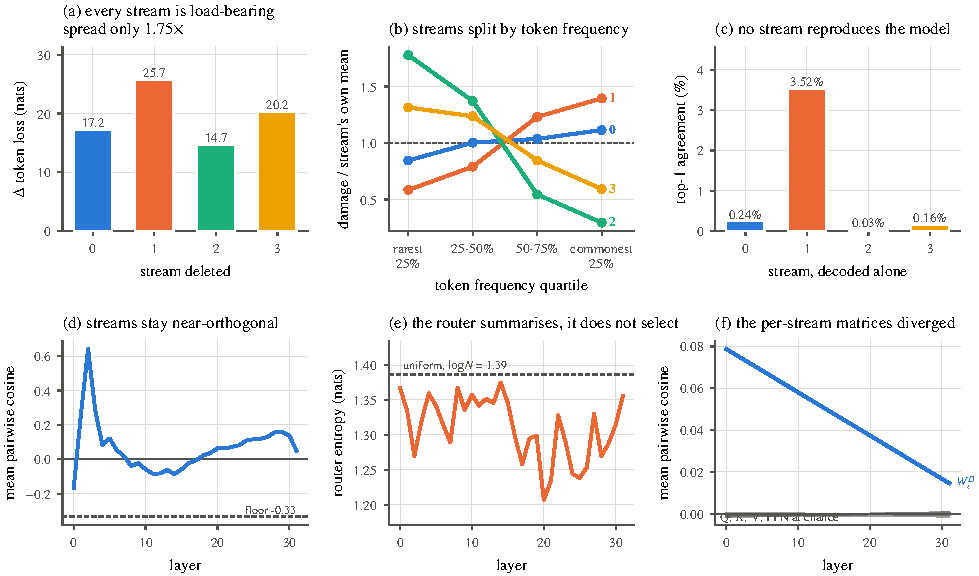
\includegraphics[width=\textwidth]{fig_analysis.pdf}
\end{center}
\caption{Stream-level analysis of the $L{=}32$ model. \textbf{(a)} deleting any
stream destroys the model, and the spread across streams is only $1.75\times$.
\textbf{(b)} normalising each stream by its own mean reveals a monotonic split
along token frequency: streams 2 and 3 carry rare tokens, streams 0 and 1 carry
common ones. \textbf{(c)} decoded alone, no stream reproduces more than $3.5\%$
of the model's predictions. \textbf{(d,e)} activation similarity and router
entropy per layer, against the $-1/(\nsub{-}1)$ floor and $\log\nsub$.
\textbf{(f)} in weight space the per-stream attention and FFN matrices are
uncorrelated at every depth, while the distribute matrices share a small
component that decays with depth.}
\label{fig:subablate}
\end{figure}

\paragraph{Device parallelism.} Streams have no within-layer cross-stream data
dependency, so the $\nsub$ columns of a layer can be placed on different devices
with a single $\dsub$-wide all-reduce at the coupling. That exchange is narrower
than the two $\dmodel$-wide all-reduces per layer of tensor parallelism
\citep{shoeybi2021megatron}, and it avoids the all-to-all token dispatch that
expert parallelism requires. \TODO{optional: measured 2-GPU numbers}

% =========================================================================
\section{Limitations}
\label{sec:limitations}
% =========================================================================

\textbf{Range of validity.} The efficiency multipliers of Table~\ref{tab:ratio}
are measured from 199M to 914M total parameters and $7.6\times10^{17}$ to
$2.4\times10^{19}$ training FLOPs. Below roughly 100M parameters MST is
\emph{worse} than dense on the compute axes: the coupling and input/output
projections are a fixed overhead that has not yet amortized. We observe no
crossover at the upper end and the multiplier is flat to mildly increasing, but we
cannot exclude a crossover beyond 914M. This caution is not hypothetical: MoL
reports an advantage at 104M that inverts into a 3.01 PPL deficit at 1.3B on the
iso-total-parameter axis.

\textbf{Token ratio.} All models are trained at 10.5 tokens per scaling parameter.
Partial evidence that the result is not an artifact of this ratio comes from
overtrained runs at $2.6\times$ the budget, where the ordering is preserved
\TODO{report these two points; a dense point at matched ratio would make the
claim clean}.

\textbf{Hardware utilization and decode.} MST attains half the utilization of
dense, for the two reasons decomposed in Section~\ref{sec:results}: a measured
$2.13\times$ kernel penalty intrinsic to $d_h{=}32$, and an implementation cost
we have not removed. Our wall-clock advantage is therefore smaller than our FLOP
advantage. Decode is worse still: it is the regime where per-stream dispatch is
least amortized, since there is no sequence dimension over which to hide the
$\nsub$-fold increase in kernel launches, and we measure MST slower than dense
there (Table~\ref{tab:speed}). We claim fewer FLOPs per token and faster
training; we do not claim faster inference, and a deployment dominated by
autoregressive decoding would not benefit from MST as implemented here.

\textbf{Single seed at scale.} Seed variance is characterized at $L{=}8$ only,
where it is $\sigma \le 0.0003$~\bpb\ over three seeds, two orders of magnitude
below every effect we report; the $L\ge16$ ladder is single-seed per point, as is
standard at this scale but worth stating.

\textbf{Scope.} We study pre-training perplexity and zero-shot transfer for
decoder-only language models at $T{=}2048$. We do not study instruction tuning,
long-context training, or $\nsub$ scaled jointly with $\dmodel$.

% =========================================================================
\section{Conclusion}
% =========================================================================

Narrow parallel blocks are a promising way to restructure the transformer layer,
but the way they are usually built, projecting into and out of a full-width
residual stream and paying for the projections with sparsity, gives up
total-parameter efficiency to buy active-compute efficiency. We showed that if the
narrow blocks partition the residual stream instead, the decomposition is free:
attention cost and KV cache are preserved exactly, per-layer matmul parameters
fall by $\nsub$, no dispatch machinery is needed, and the resulting dense model
dominates a strongly-tuned dense baseline on parameters, inference FLOPs and
training compute at once. The remaining design question is not how to route, but
how much the columns must talk. Our evidence is that they must talk, and that
almost any way of doing so works equally well.

% =========================================================================
% Required / recommended statements. These sit before the references and do
% not count toward the page limit.
% =========================================================================

\subsection*{AI use statement}

Generative AI tools were used in this work as a coding and drafting assistant.
Specifically: (i) implementation support for the architecture, training and
evaluation code; (ii) analysis scripts that recompute the parameter and FLOP
accounting reported in Table~\ref{tab:cost} and fit the scaling laws in
Table~\ref{tab:fits}; (iii) figure generation; and (iv) drafting and editing of
the manuscript text. \TODO{authors: confirm or amend this list, and add any use
not covered, e.g. literature search or idea generation}

Generative AI was not used to generate or alter any experimental result. All
numbers reported in this paper come from training runs and from deterministic
accounting code executed by the authors; no measurement was produced, imputed or
edited by a language model. All AI-assisted code was read, executed and checked
against independent references by the authors: the parameter and FLOP accounting
was verified against the closed-form derivation of Appendix~\ref{app:budget},
and the scaling fits were reproduced from the raw run table. The authors have
reviewed all AI-assisted text and take full responsibility for the final content
of this work, including all text, claims and artifacts.

\subsection*{Ethics statement}

This work studies the pre-training efficiency of decoder-only language models.
It involves no human subjects, no personally identifying data and no user study.
Training data is a publicly released filtered web corpus \citep{penedo2024fineweb};
we introduce no new dataset and release none. The models trained here are small
by contemporary standards, are not instruction-tuned or deployed, and are not
intended or suitable for downstream use; they inherit whatever biases are present
in the underlying corpus, and we make no claim that they are safe for
application. The contribution is architectural, and its foreseeable effect is to
reduce the parameter count and compute required to reach a given language
modelling quality. We regard the primary societal consideration as the standard
dual-use property of any efficiency result: the same reduction that lowers the
cost of research also lowers the cost of producing capable models. We see no
concern specific to this architecture beyond that general property. The authors
declare no conflicts of interest.

\subsection*{Reproducibility statement}

The architecture is specified completely in Section~\ref{sec:method}: the
per-stream sublayers, the coupling of Eq.~\ref{eq:coupling}, the geometric
window assignment of Section~\ref{sec:windows}, and the two optimizer
modifications of Section~\ref{sec:optim}, with the term-by-term parameter budget
in Appendix~\ref{app:budget}. Section~\ref{sec:experiments} fixes the model
ladder ($\dmodel = 64L$ rounded to a multiple of 128, $\nsub{=}4$, $T{=}2048$),
the token budget rule (10.5 tokens per scaling parameter, where scaling
parameters are transformer matrices plus the output head), and the fact that the
dense baseline shares every component and hyper-parameter with MST except the
layer structure. Full hyper-parameters and per-run configurations are in
Appendix~\ref{app:details}.

Two points bear directly on reproducing the numbers. First, all cost columns in
Table~\ref{tab:cost} are recomputed for both arms from a single implementation
at one commit rather than taken from the original run logs, so the two arms are
comparable to each other; the accounting script and the resulting table are
released with the code. Second, the ablations of Section~\ref{sec:ablations} are
run at $L{=}8$ with three seeds and we report the seed spread, while the
$L\ge16$ ladder is single-seed per point; Table~\ref{tab:transfer} gives the
evidence we have that the $L{=}8$ ordering transfers.
\TODO{authors: add the code/artifact URL once anonymised, and state the exact
commit}

\bibliography{mst}
\bibliographystyle{iclr2027_conference}

\appendix
% =========================================================================
\section{Per-layer parameter budget}
\label{app:budget}
% =========================================================================

Term by term, for one layer at width $\dmodel$ with $\nsub$ streams of width
$\dsub=\dmodel/\nsub$. This is the derivation behind Eq.~\ref{eq:budget}.

\begin{table}[h]
\caption{Per-layer parameter budget. The $\nsub$ sub-transformers cost $12\dmodel^2/\nsub$
and the coupling costs a further $3\dmodel^2/\nsub$, so a layer costs $15\dmodel^2/\nsub$
against $12\dmodel^2$ dense: a reduction of $0.8\nsub$, not $\nsub$. The router term
$\nsub\dsub$ is $0.02\%$ of the layer at $\dmodel{=}512$ and is omitted from the totals.}
\label{tab:budget}
\begin{center}
\begin{small}
\begin{tabular}{llll}
\toprule
Component & Shapes & Parameters & At $\nsub{=}4$ \\
\midrule
Attention, $\nsub$ subs & $4\times(\dsub\!\times\!\dsub)$ each & $4\dmodel^2/\nsub$ & $1.00\,\dmodel^2$ \\
FFN, $\nsub$ subs       & $(4\dsub\!\times\!\dsub)+(\dsub\!\times\!4\dsub)$ each & $8\dmodel^2/\nsub$ & $2.00\,\dmodel^2$ \\
Coupling bottleneck     & $(\dmodel\!\times\!\dsub)+(\dsub\!\times\!\dmodel)$ & $2\dmodel^2/\nsub$ & $0.50\,\dmodel^2$ \\
Coupling scatter        & $\nsub\times(\dsub\!\times\!\dsub)$ & $\dmodel^2/\nsub$ & $0.25\,\dmodel^2$ \\
Coupling router         & $\nsub\!\times\!\dsub$ & $\nsub\dsub$ & $\approx 0$ \\
\midrule
\textbf{MST layer}      &  & $\mathbf{15\dmodel^2/\nsub}$ & $\mathbf{3.75\,\dmodel^2}$ \\
Dense layer             & $4\times(\dmodel\!\times\!\dmodel) + 8\dmodel^2$ & $12\dmodel^2$ & $12.00\,\dmodel^2$ \\
\midrule
\textbf{Reduction}      &  & $\mathbf{0.8\nsub}$ & $\mathbf{3.20\times}$ \\
\bottomrule
\end{tabular}
\end{small}
\end{center}
\end{table}

% =========================================================================
\section{Coupling variants that did not help}
\label{app:negative}
% =========================================================================

Every variant below was run on top of the full recipe of
Section~\ref{sec:optim} at $L{=}8$, three seeds each. None improved on the
routed bottleneck of Eq.~\ref{eq:coupling}. We report them because the pattern is
itself the finding: the coupling must exist, but its form is close to irrelevant.

\begin{table}[h]
\caption{Coupling variants that did not improve on the routed bottleneck, $L{=}8$.}
\label{tab:negative}
\begin{center}
\begin{small}
\begin{tabular}{llcll}
\toprule
Hypothesis & Variant & $\Delta$ \bpb & Variant & $\Delta$ \bpb \\
\midrule
Needs nonlinearity   & SiLU bottleneck & \PH & Concat--MLP--split & \PH \\
Needs finer routing  & Per-slice routing & \PH & Input-gated router & \PH \\
Needs memory         & Multi-layer lookback & \PH & Hyper-connected residual & \PH \\
Needs 2nd order      & Bilinear aggregate & \PH & Cross-sub FFN gating & \PH \\
Attention needs cross-sub & Cross-sub KV injection & \PH & Low-rank query modulation & \PH \\
Features stuck in one sub & Cyclic feature permutation & \PH & Global residual stream & \PH \\
\bottomrule
\end{tabular}
\end{small}
\end{center}
\end{table}

% =========================================================================
\section{Additional ablations}
\label{app:extra}
% =========================================================================

\begin{table}[h]
\caption{Rows omitted from Table~\ref{tab:ablation}: the two optimizer
interventions applied separately, and the transition bottleneck width sweep.
$L{=}8$, three seeds.}
\begin{center}
\begin{small}
\begin{tabular}{llcc}
\toprule
& Condition & \bpb & $\Delta$ \\
\midrule
\multirow{2}{*}{Optimizer, separately}
 & Block-diagonal Muon only & \PH & \PH \\
 & Per-sub LR only          & \PH & \PH \\
\midrule
\multirow{3}{*}{Bottleneck width}
 & $\times 1$ ($\dsub$)   & \PH & \PH \\
 & $\times 2$             & \PH & \PH \\
 & $\times 4$ ($\dmodel$) & \PH & n/a \\
\bottomrule
\end{tabular}
\end{small}
\end{center}
\end{table}

% =========================================================================
\section{Experimental details}
\label{app:details}
% =========================================================================
\TODO{full hyper-parameters; per-run configuration hashes; extended ablation
table; FLOP accounting derivation; seed-variance table}

\end{document}